\documentclass[11pt,]{article}
\usepackage[]{mathpazo}
\usepackage{amssymb,amsmath}
\usepackage{ifxetex,ifluatex}
\usepackage{fixltx2e} % provides \textsubscript
\ifnum 0\ifxetex 1\fi\ifluatex 1\fi=0 % if pdftex
  \usepackage[T1]{fontenc}
  \usepackage[utf8]{inputenc}
\else % if luatex or xelatex
  \ifxetex
    \usepackage{mathspec}
  \else
    \usepackage{fontspec}
  \fi
  \defaultfontfeatures{Ligatures=TeX,Scale=MatchLowercase}
\fi
% use upquote if available, for straight quotes in verbatim environments
\IfFileExists{upquote.sty}{\usepackage{upquote}}{}
% use microtype if available
\IfFileExists{microtype.sty}{%
\usepackage{microtype}
\UseMicrotypeSet[protrusion]{basicmath} % disable protrusion for tt fonts
}{}
\usepackage[margin = 1in]{geometry}
\usepackage{hyperref}
\hypersetup{unicode=true,
            pdftitle={Postsecondary and Workforce Readiness Reports},
            pdfborder={0 0 0},
            breaklinks=true}
\urlstyle{same}  % don't use monospace font for urls
\usepackage{longtable,booktabs}
\usepackage{graphicx,grffile}
\makeatletter
\def\maxwidth{\ifdim\Gin@nat@width>\linewidth\linewidth\else\Gin@nat@width\fi}
\def\maxheight{\ifdim\Gin@nat@height>\textheight\textheight\else\Gin@nat@height\fi}
\makeatother
% Scale images if necessary, so that they will not overflow the page
% margins by default, and it is still possible to overwrite the defaults
% using explicit options in \includegraphics[width, height, ...]{}
\setkeys{Gin}{width=\maxwidth,height=\maxheight,keepaspectratio}
\IfFileExists{parskip.sty}{%
\usepackage{parskip}
}{% else
\setlength{\parindent}{0pt}
\setlength{\parskip}{6pt plus 2pt minus 1pt}
}
\setlength{\emergencystretch}{3em}  % prevent overfull lines
\providecommand{\tightlist}{%
  \setlength{\itemsep}{0pt}\setlength{\parskip}{0pt}}
\setcounter{secnumdepth}{0}
% Redefines (sub)paragraphs to behave more like sections
\ifx\paragraph\undefined\else
\let\oldparagraph\paragraph
\renewcommand{\paragraph}[1]{\oldparagraph{#1}\mbox{}}
\fi
\ifx\subparagraph\undefined\else
\let\oldsubparagraph\subparagraph
\renewcommand{\subparagraph}[1]{\oldsubparagraph{#1}\mbox{}}
\fi

%%% Use protect on footnotes to avoid problems with footnotes in titles
\let\rmarkdownfootnote\footnote%
\def\footnote{\protect\rmarkdownfootnote}

%%% Change title format to be more compact
\usepackage{titling}

% Create subtitle command for use in maketitle
\newcommand{\subtitle}[1]{
  \posttitle{
    \begin{center}\large#1\end{center}
    }
}

\setlength{\droptitle}{-2em}
  \title{Postsecondary and Workforce Readiness Reports}
  \pretitle{\vspace{\droptitle}\centering\huge}
  \posttitle{\par}
\subtitle{Random District}
  \author{}
  \preauthor{}\postauthor{}
  \predate{\centering\large\emph}
  \postdate{\par}
  \date{April 12, 2017}


\begin{document}
\maketitle

\section{Cover page}\label{cover-page}

\section{Random District}\label{random-district}

\subsection{List of School Names}\label{list-of-school-names}

\begin{center}\rule{0.5\linewidth}{\linethickness}\end{center}

This page will contain a series of figures that in a clean way display
for the most recent cohort. It will act as an introduction for the lay
viewer. What are the key pieces of data that the state is monitoring and
how does your school/district perform.

\begin{itemize}
\tightlist
\item
  Percent of most recent graduates who enrolled in any postsecondary
  institution
\item
  Percent of most recent graduates who enrolled in any postsecondary
  institution, by type of PS institution
\item
  Percent of most recent graduates concentrating in CTE
\item
  Average ACT scores 
\end{itemize}

\textbf{Most Common Insitutions}

\begin{longtable}[]{@{}lr@{}}
\toprule
Institution Name & Number of Enrollees\tabularnewline
\midrule
\endhead
Jackson State Community College & 63\tabularnewline
Tennessee Technology Center at Whiteville & 17\tabularnewline
University of Memphis & 15\tabularnewline
Middle Tennessee State University & 12\tabularnewline
University of Tennessee, Martin & 7\tabularnewline
\bottomrule
\end{longtable}

\subsection{Overview of what we want to
show.}\label{overview-of-what-we-want-to-show.}

\newpage

\subsubsection{Definitions}\label{definitions}

\textbf{Graduation Year}: This report uses the term Graduation Year to
monitor a cohort of students. This set of graduates would align with the
On-Time Graduates with a regular diploma, based on when the group of
students entered high school. For example, this report provides data on
the 2011 freshman cohort, which is a group of students who entered high
school in the fall of 2011. The vast majority of these students
graduated in the spring of 2015. The most recent postsecondary
enrollment data available is for the 2015 graduates fromn the 2011
freshman cohor.

\textbf{Postsecondary Enrollment}: A student is identified as having
enrolled in a postsecondary institution if they enroll within 12 months
of expectred graduation year for students in the 2011 ninth grade
cohort. Eligible institutions include Tennessee Board of Regents'
schools, UT System, Tennessee Colleges of Applied Technology, TICUA
institutions, and any non-Tennessee institution that shares enrollment
information with the National Student Clearinghouse.

\textbf{Postsecondary Remediation}: A student is identified as being
assigned to a remedial course if they are designated as having non-zero
remedial hours by their postsecondary institution. This information is
only available from Tennessee public postsecondary institutions. At this
time, the data are not able to be disaggregated at the subject level
(e.g.~we are unable to see whether a student took a remedial course in
English or Math).

\textbf{Postsecondary Completion}: Postsecondary completion
documentation is shown for students in the 2007 and 2008 ninth grade
graduating cohorts, the earliest group of students that the Tennessee
Longitudinal Data System can track from secondary into postsecondary.
Any degree-granting public institution that submits completion
information to THEC is included in this set of data points. For students
in the 2007 ninth grade cohort, we display a 5 year completion rate and
for students in the 2008 ninth grade cohort, we show a 4 year completion
rate. As of April 12, 2017, the most recent term with completion
information available is Summer 2016. A student's most advanced degree
is shown.

\subsubsection{District comparisons}\label{district-comparisons}

For some topics, comparing a school district's data to statewide trends
is not illuminating because the characteristics of the district's
student population are very different from the characteristics of the
student population across Tennessee. For ACT and postsecondary
enrollment data, this report provides comparisons to Tennessee school
districts whose populations share similar demographic characteristics.
Be respectful in your use of other school districts' information; do not
share this information publicly.

\begin{longtable}[]{@{}lccccc@{}}
\toprule
\begin{minipage}[b]{0.17\columnwidth}\raggedright\strut
Your District\strut
\end{minipage} & \begin{minipage}[b]{0.13\columnwidth}\centering\strut
Comparison 1\strut
\end{minipage} & \begin{minipage}[b]{0.13\columnwidth}\centering\strut
Comparison 2\strut
\end{minipage} & \begin{minipage}[b]{0.13\columnwidth}\centering\strut
Comparison 3\strut
\end{minipage} & \begin{minipage}[b]{0.13\columnwidth}\centering\strut
Comparison 4\strut
\end{minipage} & \begin{minipage}[b]{0.13\columnwidth}\centering\strut
Comparison 5\strut
\end{minipage}\tabularnewline
\midrule
\endhead
\begin{minipage}[t]{0.17\columnwidth}\raggedright\strut
Random District\strut
\end{minipage} & \begin{minipage}[t]{0.13\columnwidth}\centering\strut
Fayette County\strut
\end{minipage} & \begin{minipage}[t]{0.13\columnwidth}\centering\strut
Lauderdale County\strut
\end{minipage} & \begin{minipage}[t]{0.13\columnwidth}\centering\strut
Haywood County\strut
\end{minipage} & \begin{minipage}[t]{0.13\columnwidth}\centering\strut
Dyersburg City\strut
\end{minipage} & \begin{minipage}[t]{0.13\columnwidth}\centering\strut
Jackson-Madison County\strut
\end{minipage}\tabularnewline
\bottomrule
\end{longtable}

\newpage

\paragraph{Key questions}\label{key-questions}

\begin{itemize}
\tightlist
\item
  What are the general enrollment trends in my district?
\end{itemize}

\begin{center}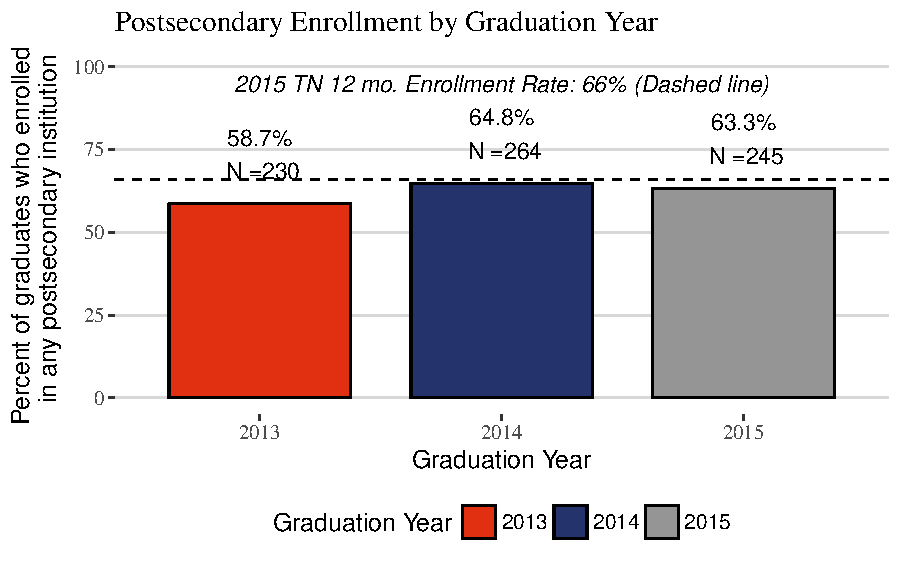
\includegraphics{20170411_PSWRR_no_CTE_files/figure-latex/Enrollment over time-1} \end{center}

\begin{itemize}
\item
  What type of institutions are my students enrolling in?
\item
  Percent of graduates who enrolled, by type of institution
\end{itemize}

\begin{center}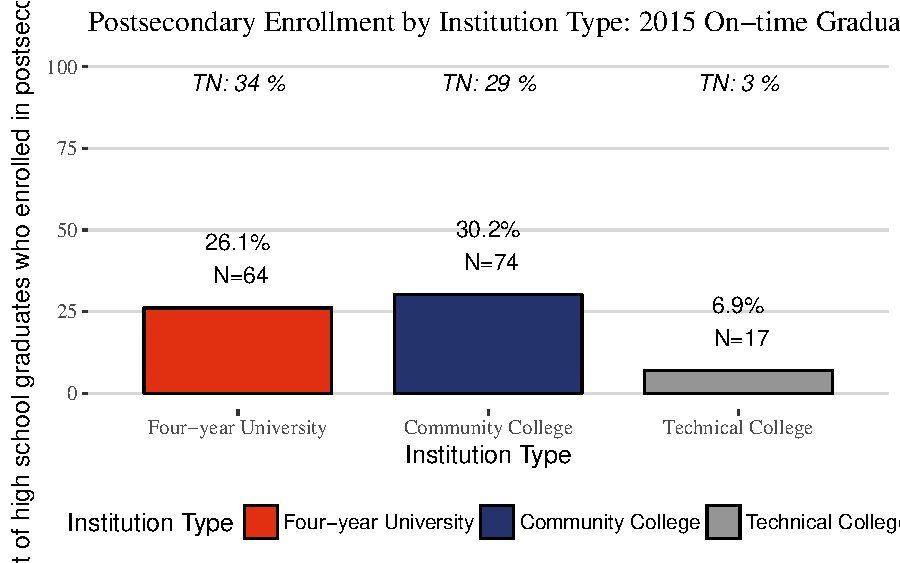
\includegraphics{20170411_PSWRR_no_CTE_files/figure-latex/District by Type-1} \end{center}

\newpage

\textbf{District Comparisons}

\paragraph{Key Questions}\label{key-questions-1}

\begin{itemize}
\tightlist
\item
  How does the overall enrollment compare to similar districts in terms
  of overall postsecondary enrollment?
\item
  How does the overall enrollment compare to the state overall
  enrollment?
\item
  How does the enrollment into different institution types compare to
  similar districts in terms of overall postsecondary enrollment?
\item
  How does the enrollment into different institution types compare to
  the state distribution of enrollment into institution types?
\end{itemize}

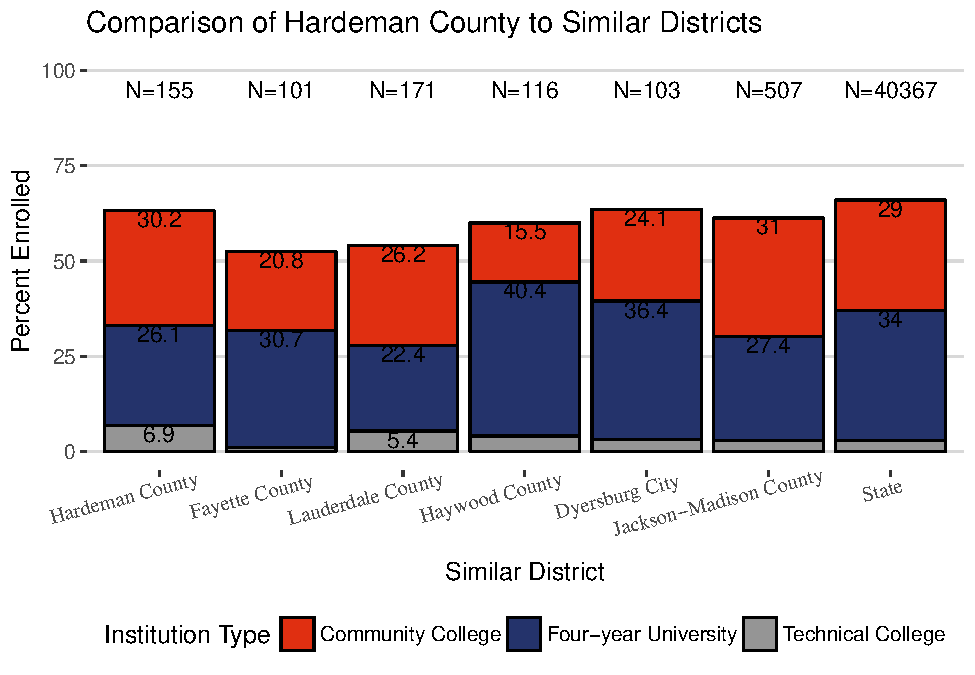
\includegraphics{20170411_PSWRR_no_CTE_files/figure-latex/comparison_districts-1.pdf}

\begin{longtable}[]{@{}lrrr@{}}
\toprule
Similar District & Community College & Four-year University & Technical
College\tabularnewline
\midrule
\endhead
Hardeman County & 30.2 & 26.1 & 6.9\tabularnewline
Fayette County & 20.8 & 30.7 & 1.0\tabularnewline
Lauderdale County & 26.2 & 22.4 & 5.4\tabularnewline
Haywood County & 15.5 & 40.4 & 4.1\tabularnewline
Dyersburg City & 24.1 & 36.4 & 3.1\tabularnewline
Jackson-Madison County & 31.0 & 27.4 & 2.9\tabularnewline
State & 29.0 & 34.0 & 3.0\tabularnewline
\bottomrule
\end{longtable}

\begin{itemize}
\tightlist
\item
  How does the overall enrollment differ across schools in my district?
\item
  How does the distribution of students to different institution types
  compare across schools in my district?
\end{itemize}

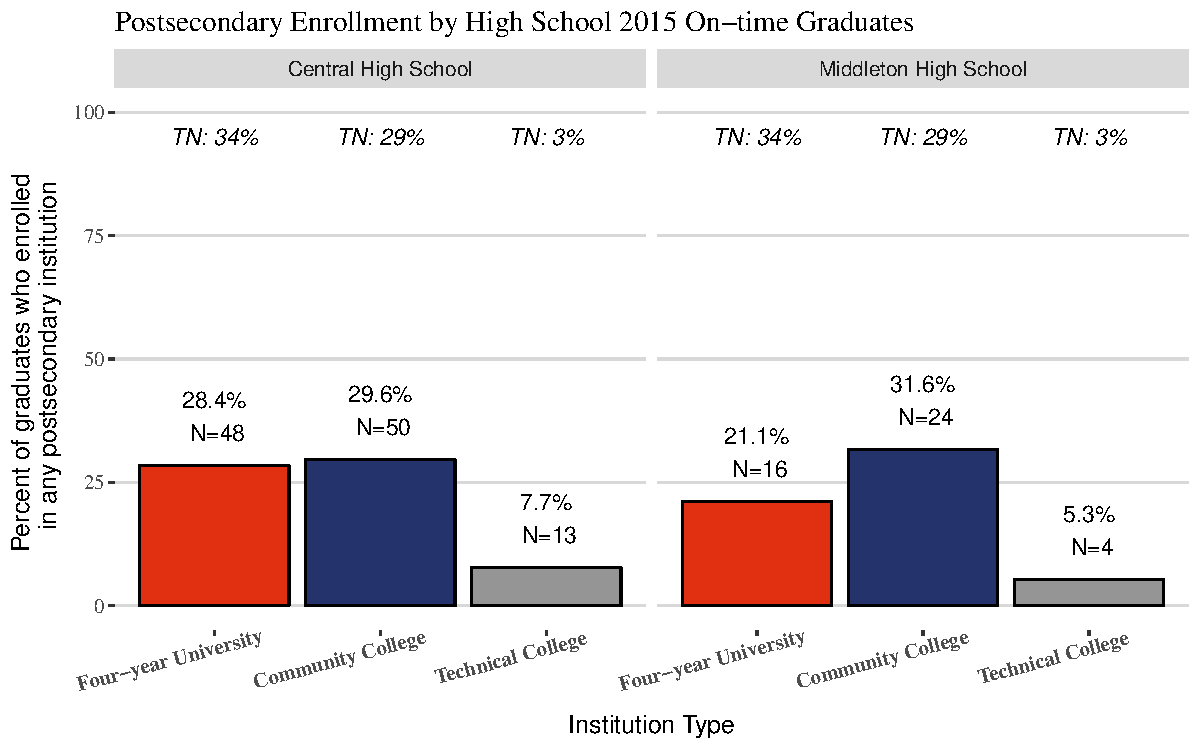
\includegraphics{20170411_PSWRR_no_CTE_files/figure-latex/Enrollment by School-1.pdf}

\newpage

\subsection{Most Common Institutions}\label{most-common-institutions}

The following table shows the most common institutions that students
from the 2015 graduating class enrolled in within 12 months of
graduation.

Consider opportunities for an external partnership with the institution
and where students have been successful. Some questions that you may
want to consider:

\begin{itemize}
\tightlist
\item
  Are students enrolling in institutions that are nearest to your
  school?
\item
  Have students taken dual enrollment courses or attended summer
  programs at these institutions while in high school?
\item
  Are students in your school aware of the majors offered at these
  institutions?
\item
  Do your programs of study align with opportunities at these
  institutions?
\end{itemize}

\begin{longtable}[]{@{}lr@{}}
\toprule
Institution Name & Number of Enrollees\tabularnewline
\midrule
\endhead
Jackson State Community College & 63\tabularnewline
Tennessee Technology Center at Whiteville & 17\tabularnewline
University of Memphis & 15\tabularnewline
Middle Tennessee State University & 12\tabularnewline
University of Tennessee, Martin & 7\tabularnewline
Tennessee State University & 6\tabularnewline
Mississippi State University & 6\tabularnewline
\bottomrule
\end{longtable}

\subsection{SECTION II: Postsecondary Enrollment by Subgroup (Most
recent year
only)}\label{section-ii-postsecondary-enrollment-by-subgroup-most-recent-year-only}

\paragraph{Key Questions}\label{key-questions-2}

\begin{itemize}
\tightlist
\item
  To what extent do we see overall equitable access by race in the same
  school to postsecondary institutions?
\item
  Within each school, to what extent are students of different racial
  backgrounds enrolling in different types of postsecondary institutions
  (e.g.~a higher distribution of one group is enrolling in four-year
  universities than two year institutions)?
\item
  If your district has more than one school, to what extent do the
  overall enrollment rates differ across schools in your districts for
  racial and ethnic groups?
\item
  If your district has more than one school, to what extent do
  enrollment rates for racial and ethnic subggroups into different types
  of postecondary institutions differ across schools?
\item
  Given this information, do you feel that all students are receiving
  the same opportunities in your district?
\end{itemize}

\begin{center}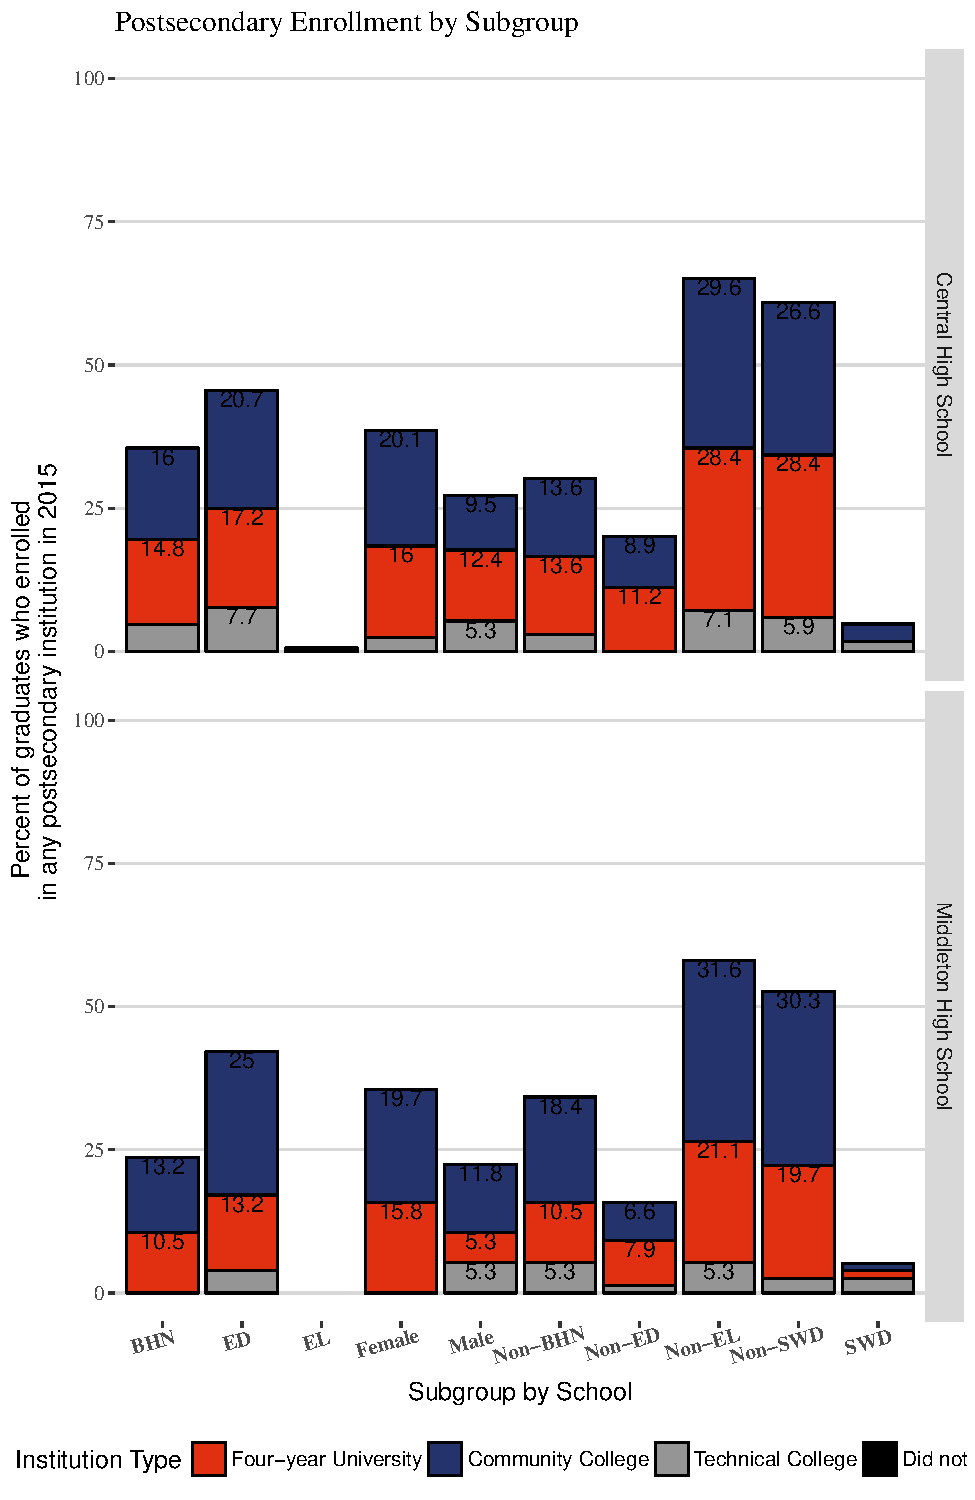
\includegraphics{20170411_PSWRR_no_CTE_files/figure-latex/subgroup Enrollment-1} \end{center}

\begin{itemize}
\tightlist
\item
  Economic Disadvantage (School level)

  \begin{itemize}
  \tightlist
  \item
    To what extent do we see equitable access by level of economic
    disadvantage in my district to postsecondary institutions? Given
    this information, do you feel that all students are receiving the
    same opportunities in your district?
  \end{itemize}
\end{itemize}

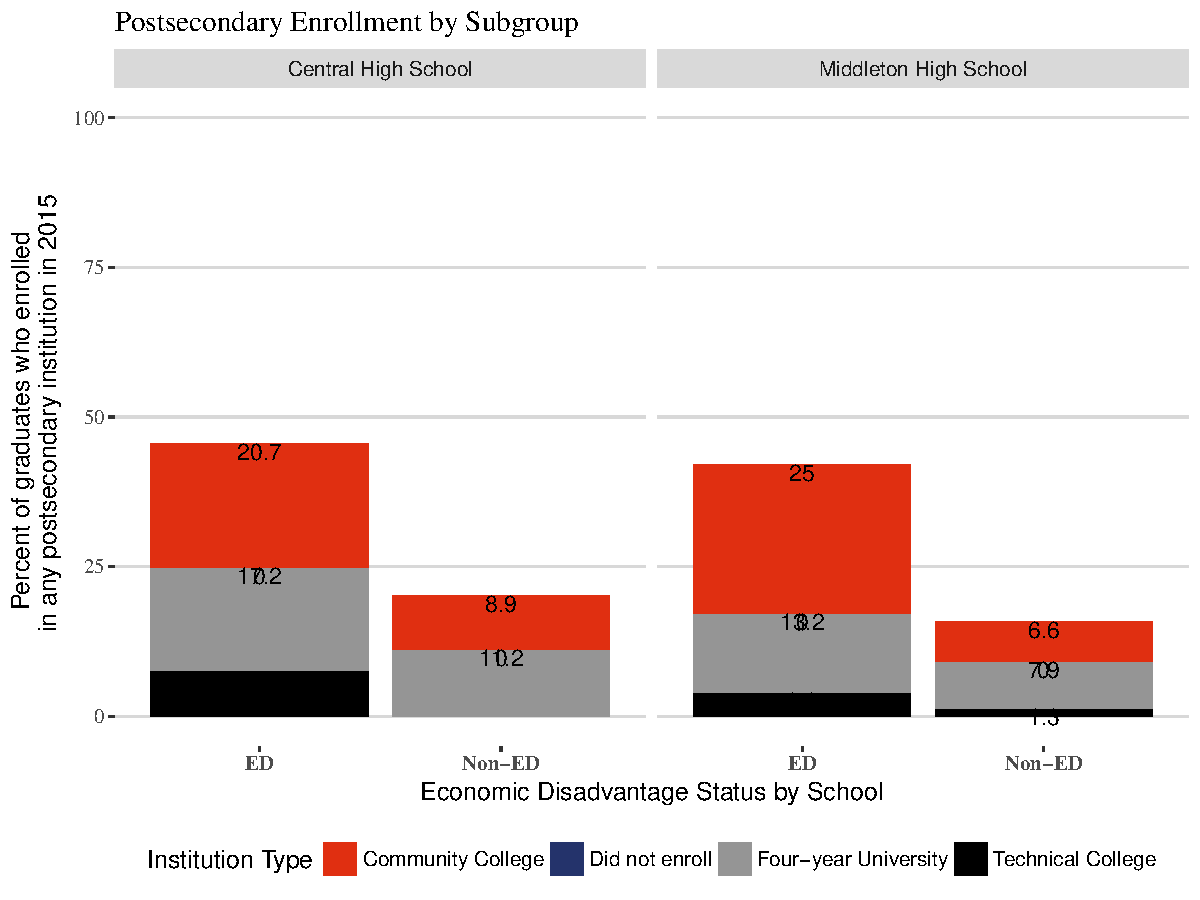
\includegraphics{20170411_PSWRR_no_CTE_files/figure-latex/Figure5c-1.pdf}

\newpage

\subsection{Postsecondary Enrollment By Academic Achievement (Most
recent year
only)}\label{postsecondary-enrollment-by-academic-achievement-most-recent-year-only}

\paragraph{Key Questions}\label{key-questions-3}

\begin{itemize}
\item
  Consider the distribution of ACT composite scores for the students in
  your district.
  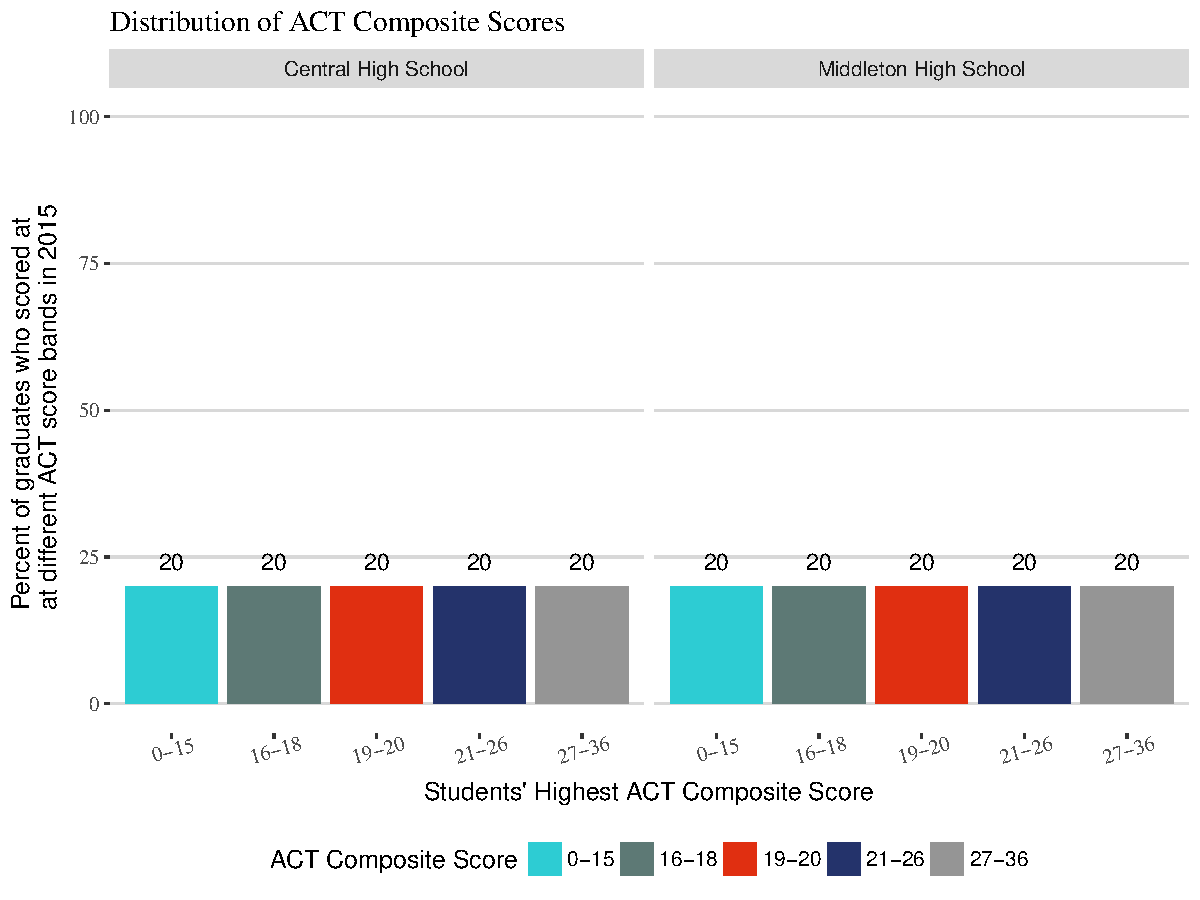
\includegraphics{20170411_PSWRR_no_CTE_files/figure-latex/Figure7aa-1.pdf}
\item
  Overall Enrollment By ACT Scores (State Comparison, District, and
  school level) The above figure displays the distribution of ACT
  scores. That group of students becomes the denominator for the next
  figure that shows postsecondary enrollment rates at each ACT score
  band. Thus, if a school had 50 students score between a 19-20, and 40
  of those students enrolled in a postsecondary institution, the overall
  enrollment for that score band would be 80\%.

  \begin{itemize}
  \tightlist
  \item
    To what extent do ACT Scores relate to the postsecondary enrollment
    of the students in my district?
  \end{itemize}
\end{itemize}

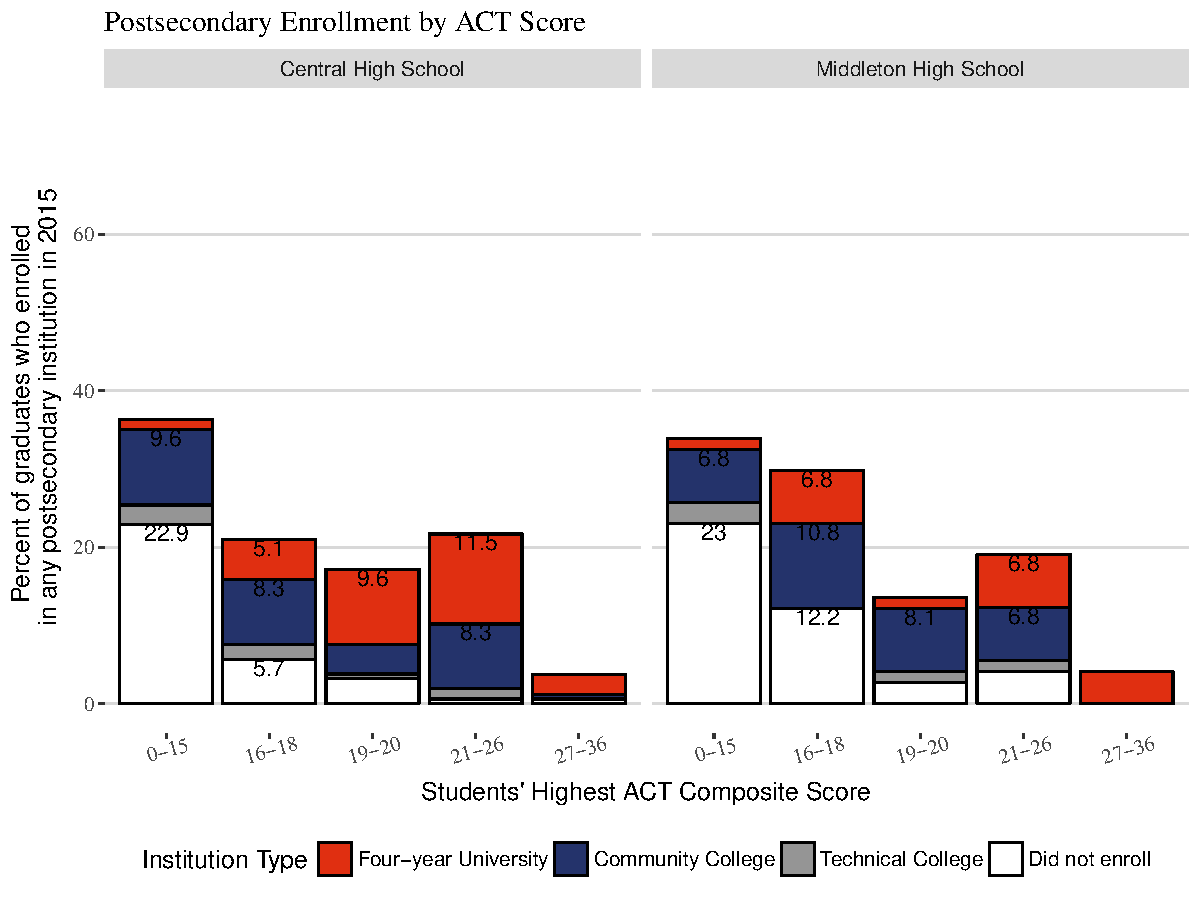
\includegraphics{20170411_PSWRR_no_CTE_files/figure-latex/Figure7a-1.pdf}

\begin{itemize}
\tightlist
\item
  Other possible questions

  \begin{itemize}
  \tightlist
  \item
    To what extent does the relationship between ACT scores and
    postsecondary enrollment in your district differ from the state
    average?
  \item
    To what extent does the relationship between ACT scores and the type
    of postsecondary institution where students are enrolling in your
    district differ from the state average?
  \end{itemize}
\end{itemize}

\newpage

\subsection{Postsecondary Enrollment By Coursework (Most recent year
only)}\label{postsecondary-enrollment-by-coursework-most-recent-year-only}

\paragraph{Key questions}\label{key-questions-4}

\begin{itemize}
\tightlist
\item
  To what extent do all students have access to rigorous coursework that
  can result in early postsecondary credit in the 2011 graduating cohort
  who graduated in spring 2015?
\end{itemize}

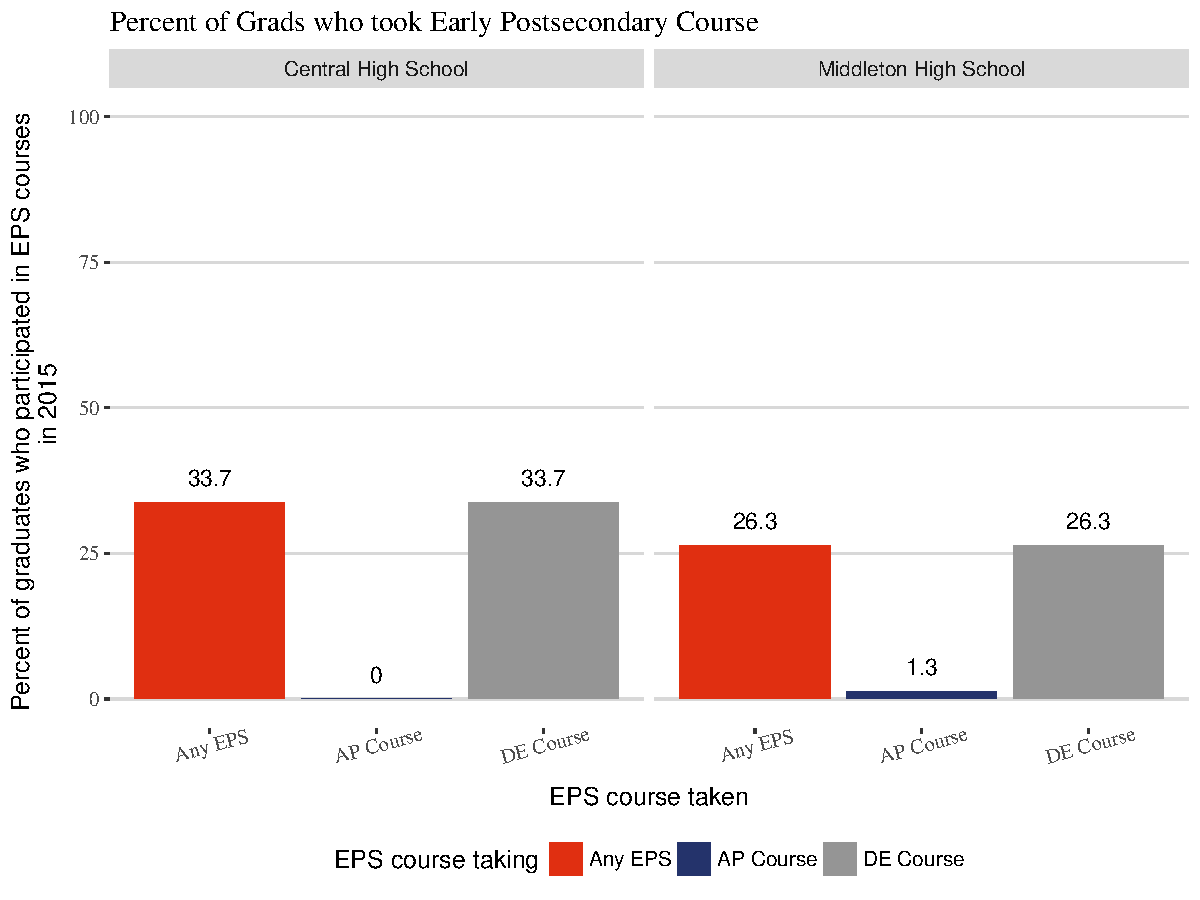
\includegraphics{20170411_PSWRR_no_CTE_files/figure-latex/Figure9a-1.pdf}

\begin{itemize}
\tightlist
\item
  To what extent does access to EPS courses differ by student race?
\end{itemize}

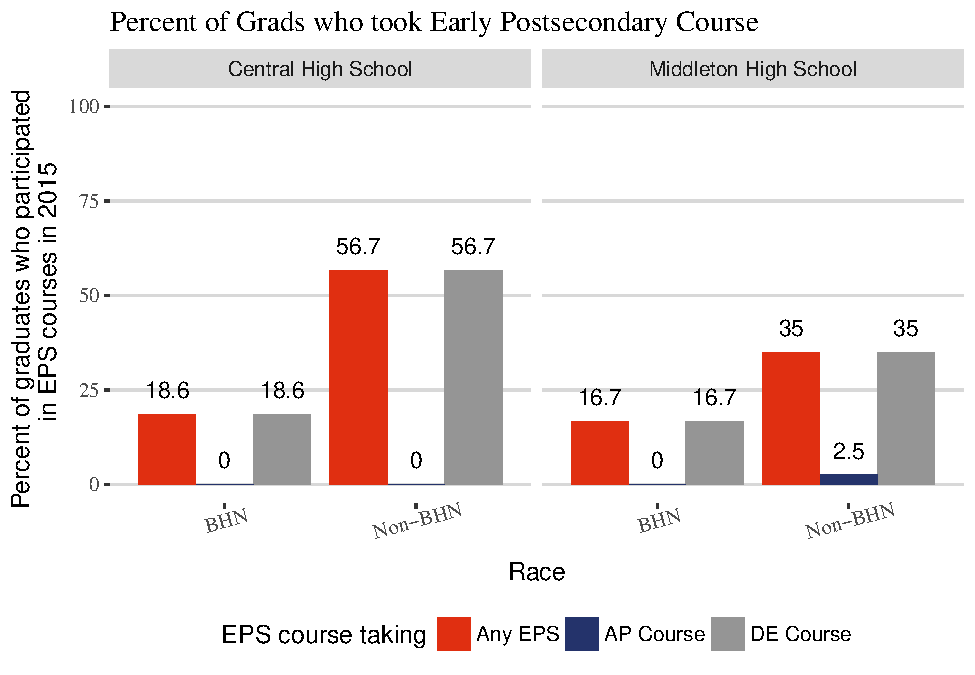
\includegraphics{20170411_PSWRR_no_CTE_files/figure-latex/Figure9b-1.pdf}

\begin{itemize}
\tightlist
\item
  To what extent does this differ by the economic disadvantage status of
  the students?
\end{itemize}

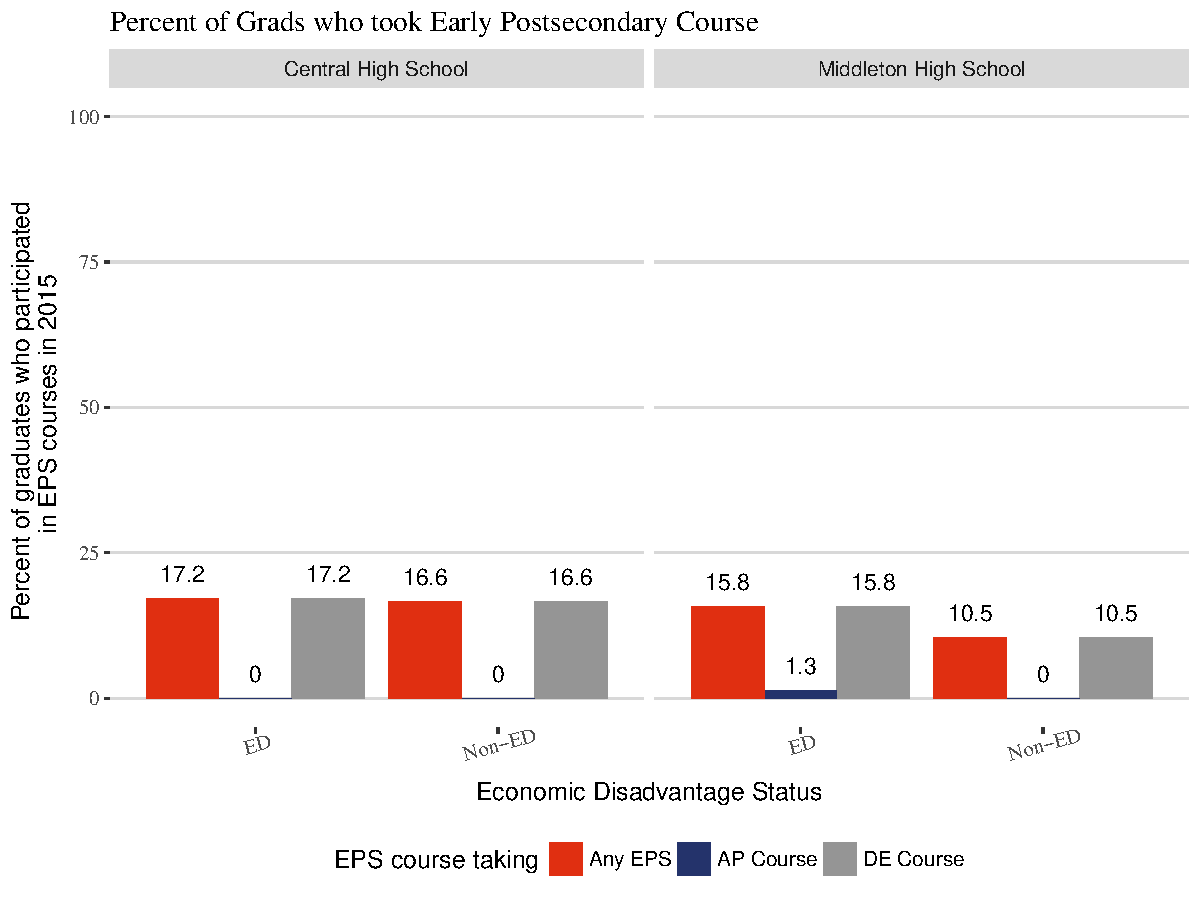
\includegraphics{20170411_PSWRR_no_CTE_files/figure-latex/Figure9c-1.pdf}

\begin{itemize}
\tightlist
\item
  To what extent do students who took EPS courses enroll in a
  postsecondary institution?
\item
  To what extent do students who took EPS courses enroll in different
  types of postsecondary institutions?
\end{itemize}

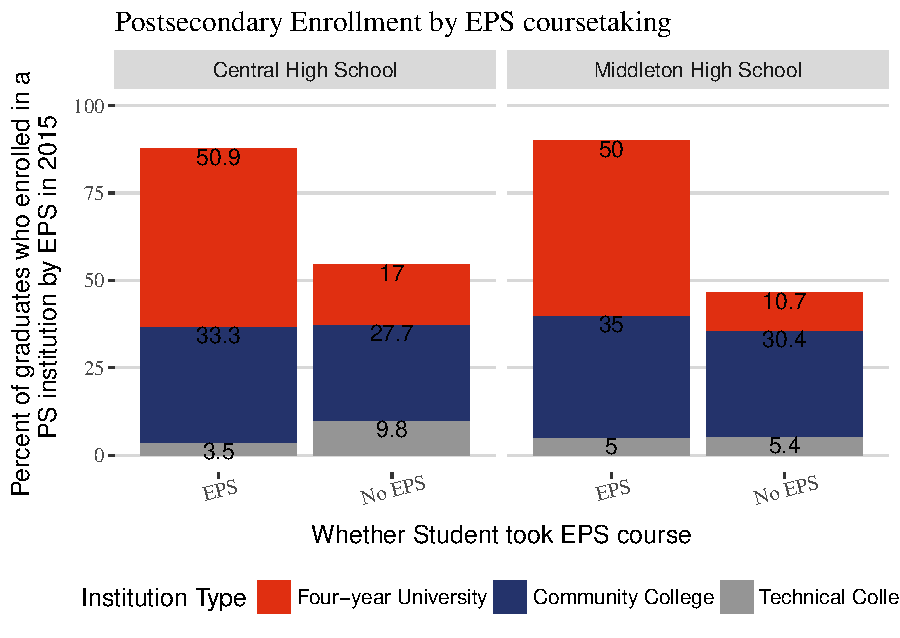
\includegraphics{20170411_PSWRR_no_CTE_files/figure-latex/Figure9d-1.pdf}

Research by the department has seen increases in postsecondary
enrollment for ED students who take early postsecondary courses.

\begin{itemize}
\tightlist
\item
  To what extent do Economically Disadvantaged students benefit from EPS
  courses?
\end{itemize}

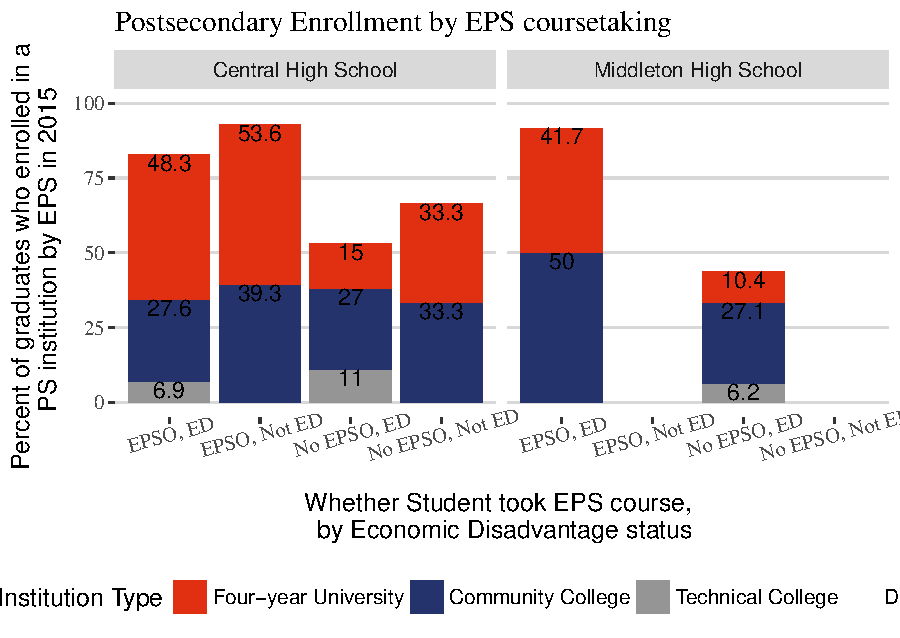
\includegraphics{20170411_PSWRR_no_CTE_files/figure-latex/Figure9e-1.pdf}

\newpage

\subsection{Persistence of all students (Not included in initial
release)}\label{persistence-of-all-students-not-included-in-initial-release}

\begin{itemize}
\tightlist
\item
  Earning 1 year worth of credits in two years
\item
  Remediation (by subject)
\item
  WILL BE INCLUDED IN INITITAL REPORT
\end{itemize}

\subsection{Completion Rates by Institution Type (5 year (2007 cohort),
4 year (2008
cohort))}\label{completion-rates-by-institution-type-5-year-2007-cohort-4-year-2008-cohort}

\newpage

\section{APPENDICES}\label{appendices}

\subsection{Appendix A: Strategies???}\label{appendix-a-strategies}

CCTE Team would develop a series of strategies that would target
potential stories that would arise from the data

\subsection{Appendix B: CTE Data}\label{appendix-b-cte-data}

For the next set of figures, we would focus on the same data that was
provided at the school and district level, but focus at the concentrator
level. We will compare across program areas where applicable.

\subsection{Appendix C: Business Rules/Data
Sources}\label{appendix-c-business-rulesdata-sources}

When we release data, we have to make sure that we clear set of business
rules defined.

\section{Preliminary timeline}\label{preliminary-timeline}

\subsubsection{April 20}\label{april-20}

Based on CORE feedback, we would put together the final mock-ups to
share within the department, to THEC, TOSS, etc Bring in communications
team for state level communication plans

\subsubsection{May 1}\label{may-1}

Integration of strategies

\subsubsection{May 15}\label{may-15}

Continuing TDOE feedback, CORE Feedback and maybe trusted partners Data
Validated

\subsubsection{June}\label{june}

To Directors for feedback, Validation period begins with CORE Data
Analysts and CTE Consultants

June 30: Deadline for receiving 2016 enrollment data from P20 for SSC
reports

\subsubsection{June/July}\label{junejuly}

CORE Data analysts set up meetings with district teams CTE trainings

\subsubsection{August}\label{august}

Superintendent Study Council Preparation


\end{document}
